\documentclass[11pt,a4paper]{article}
\usepackage[margin=23mm]{geometry}
\usepackage[T1]{fontenc}
\usepackage{lmodern,microtype}
\usepackage{amsmath,amssymb,graphicx,booktabs,tabularx}
\usepackage[hidelinks]{hyperref}
\setlength{\parindent}{0pt}
\setlength{\parskip}{5pt}
\setlength{\emergencystretch}{2em}
\renewcommand{\arraystretch}{1.15}
\title{\textbf{Week 5}\\Transformer Classification and Transfer Learning}
\author{Tuomas Huilla, Tomi Maijala}
\date{\today}
\begin{document}
\maketitle

\section{Objectives and experimental design}
This report compares the Week~1 TF--IDF logistic regression baseline with
a randomly initialized Transformer on IMDb sentiment classification and
BANKING77 intent classification. A separate transfer-learning study
compares four choices of trainable components in pretrained BERT.
The implementation is divided into data preparation, baseline,
Transformer architecture, training, transfer learning, visualization,
and report generation modules.

\subsection{Datasets and splits}
IMDb has two sentiment classes. BANKING77 contains banking queries
assigned to 77 intents~\cite{banking77}.
For each dataset, a stratified 80/20 training/validation split is created
from the official training data with seed 42. The official test split
is held out from fitting and checkpoint selection.
On the full IMDb dataset this yields 20,000 training, 5,000 validation,
and 25,000 test examples. Actual split sizes and dataset fingerprints
are saved with each run.

The optional smoke mode samples a small number of examples per class
from each split and trains for one epoch. Its outputs are kept in a
separate directory and explicitly identified in the generated results.

\subsection{Preprocessing and evaluation}
For the baseline and randomly initialized Transformer, HTML entities
are decoded, HTML tags and URLs are removed, text is lowercased, Unicode
is normalized, and whitespace is collapsed. Words and numbers are
extracted while preserving internal apostrophes and hyphens. This same
rule is used in the text-length plots, baseline tokenizer, and
Transformer vocabulary. Character statistics include punctuation and
are saved both with and without spaces.

Pretrained BERT uses its own checkpoint tokenizer on the original text.
All neural inputs are truncated and padded to 128 tokens by default.
Padding is masked in attention, and the random Transformer also masks
padding during pooling. Truncation fractions are recorded separately
for each model and split.

Accuracy and macro-averaged F1 are reported for both tasks. Binary
ROC-AUC is additionally saved for IMDb. The neural checkpoint with the
highest validation accuracy is selected; training stops after two
epochs without improvement, within a default five-epoch budget.
Test data do not determine the selected checkpoint. Results from
different datasets are compared within their respective tasks.

\section{Baseline and randomly initialized Transformer}
\subsection{TF--IDF logistic regression}
The baseline follows Week~1: up to 20,000 unigram and bigram TF--IDF
features, minimum document frequency 2, maximum document frequency
0.95, and sublinear term frequency. Vocabulary and inverse document
frequencies are fitted using training data only.
Logistic regression uses $C=1$ and at most 1,000 optimization iterations.
The IMDb binary model uses the liblinear solver. BANKING77 uses lbfgs
with a multinomial loss to support all 77 classes.

\subsection{Transformer architecture and training}
The Transformer is initialized randomly. A vocabulary of up to 20,000
entries is built exclusively from the training split, including padding
and unknown-token entries. The model has 64-dimensional embeddings,
sinusoidal positional encodings, one encoder block, four attention heads,
and a feed-forward width of 128. The encoder uses GELU activation,
pre-normalization, and a final layer normalization.

Masked mean pooling produces a sequence representation. A classification
head maps this representation through a 128-unit ReLU layer and dropout
to two logits for IMDb or 77 logits for BANKING77.
Cross-entropy loss is used for both tasks.
Optimization uses AdamW with learning rate $5\times10^{-4}$, weight decay
0.01, batch size 64, dropout 0.2, and gradient clipping at norm 1.
All model parameters are trainable.

\section{BANKING77 exploration}
Training class frequencies are plotted with all intent names.
Word and character length distributions are plotted separately.
The accompanying CSV files contain descriptive statistics and two
training queries per intent. These plots help assess class imbalance
and the length of the texts presented to the models.
Saved prediction files and per-class reports support error analysis
of closely related intents.

\section{Transfer learning and layer importance}
\subsection{Pretrained checkpoint}
The Hugging Face catalogue includes BERT, RoBERTa, and DistilBERT
architectures~\cite{models}. This implementation uses
\texttt{prajjwal1/bert-tiny} by default, a compact BERT checkpoint
with two encoder blocks and hidden width 128~\cite{berttiny}.
It makes the layer comparison practical on a CPU.
A compatible BERT checkpoint can be selected through the command line.
The resolved checkpoint revision and encoder depth are recorded.

The default layer study uses BANKING77. The same experiment can also
be run on IMDb or both datasets. Each configuration reloads the same
pretrained checkpoint and resets the random seed before initializing
the task classification head and training data order.

\clearpage
\subsection{Trainable components}
Four configurations are evaluated:
\begin{enumerate}
\item Head only: the classification layer is trained and BERT is frozen.
\item Upper block: the head and final encoder block are trained.
\item Lower block: the head and first encoder block are trained.
\item Full model: embeddings, encoder blocks, pooler, and head are trained.
\end{enumerate}
The pooler and embeddings remain frozen in both partial configurations.
Encoder blocks are numbered from the input toward the output.
The upper/lower comparison changes block position at the same block
budget. In partial runs, frozen BERT components use evaluation mode;
unfrozen encoder blocks and the classification head use training mode.
Gradients can propagate through frozen operations when needed to train
an earlier block.

All four settings use the same maximum training budget, batch size,
validation selection rule, and AdamW learning rate of
$5\times10^{-4}$ by default. The common rate controls the experiment,
but may not be optimal for every configuration.
The exact names and sizes of trainable tensors are saved for auditing.
Trainable weights are counted as
\begin{equation}
N_{\mathrm{train}} =
\sum_{p:\,\mathrm{requires\_grad}(p)}\operatorname{numel}(p).
\end{equation}

\subsection{Pareto comparison}
The horizontal axis of the Pareto plot shows trainable scalar parameters
on a logarithmic scale. The vertical axis shows classification accuracy.
Configuration $a$ dominates $b$ if
\begin{equation}
N_a\leq N_b,\qquad \mathrm{Acc}_a\geq\mathrm{Acc}_b,
\end{equation}
with at least one strict inequality. Nondominated configurations form
the measured frontier. Validation plots support configuration selection;
test plots describe held-out performance. Training time is reported
separately because weight count captures only part of computational cost.

\clearpage
% Editable results, tables, captions, and discussion from the completed report.
\section{Recorded run}

This section is generated from saved experiment outputs.

This run uses the complete official training and test splits, with a stratified validation holdout from the training data.

The random seed is 42. The device is \texttt{cpu}. The maximum training budget is 5 epochs per neural configuration, with patience 2. Batch size is 64.

\subsection{imdb results}

Training, validation, and test sizes are 20000, 5000, and 25000, respectively.

\begin{table}[htbp]\centering\small

\caption{Measured performance. Accuracies and macro-F1 are percentages. Time includes neural validation and checkpoint selection.}

\begin{tabular}{lrrrrr}\toprule

Model & Weights & Val.\ acc. & Test acc. & Test F1 & Seconds\\\midrule

baseline & 20,001 & 90.18 & 89.88 & 89.88 & 46.0\\

scratch & 1,322,178 & 81.70 & 80.77 & 80.72 & 147.3\\

\bottomrule\end{tabular}\end{table}

The randomly initialized Transformer changes test accuracy by -9.11 percentage points relative to the TF--IDF baseline. The baseline directly models word and bigram evidence, while the small Transformer learns its embeddings and contextual representation from the task training data. Input truncation and the fixed training budget may also affect the comparison. These possible explanations are not isolated causally by this experiment.

For IMDb, the baseline represents the complete cleaned review, while the Transformer sees only the initial token window. Sentiment evidence later in a review can therefore be unavailable to the Transformer. Its embeddings are learned from task data without language-model pretraining.

For \texttt{scratch}, 73.4\% of training texts exceed the input limit. The selected checkpoint is from epoch 5.

\par\medskip\noindent\begin{minipage}{\linewidth}

\paragraph{Example errors: baseline}

\begin{itemize}

\item True: neg; predicted: pos. "First off let me say, If you haven't enjoyed a Van Damme movie since bloodsport, you probably will not like this movie. Most of these movies may not have the best plots or best act..."

\item True: neg; predicted: pos. "Ben, (Rupert Grint), is a deeply unhappy adolescent, the son of his unhappily married parents. His father, (Nicholas Farrell), is a vicar and his mother, (Laura Linney), is ... wel..."

\end{itemize}

\end{minipage}\par

\par\medskip\noindent\begin{minipage}{\linewidth}

\paragraph{Example errors: scratch}

\begin{itemize}

\item True: neg; predicted: pos. "First off let me say, If you haven't enjoyed a Van Damme movie since bloodsport, you probably will not like this movie. Most of these movies may not have the best plots or best act..."

\item True: neg; predicted: pos. "I had high hopes for this one until they changed the name to 'The Shepherd : Border Patrol, the lamest movie name ever, what was wrong with just 'The Shepherd'. This is a by the nu..."

\end{itemize}

\end{minipage}\par

\begin{figure}[htbp]\centering
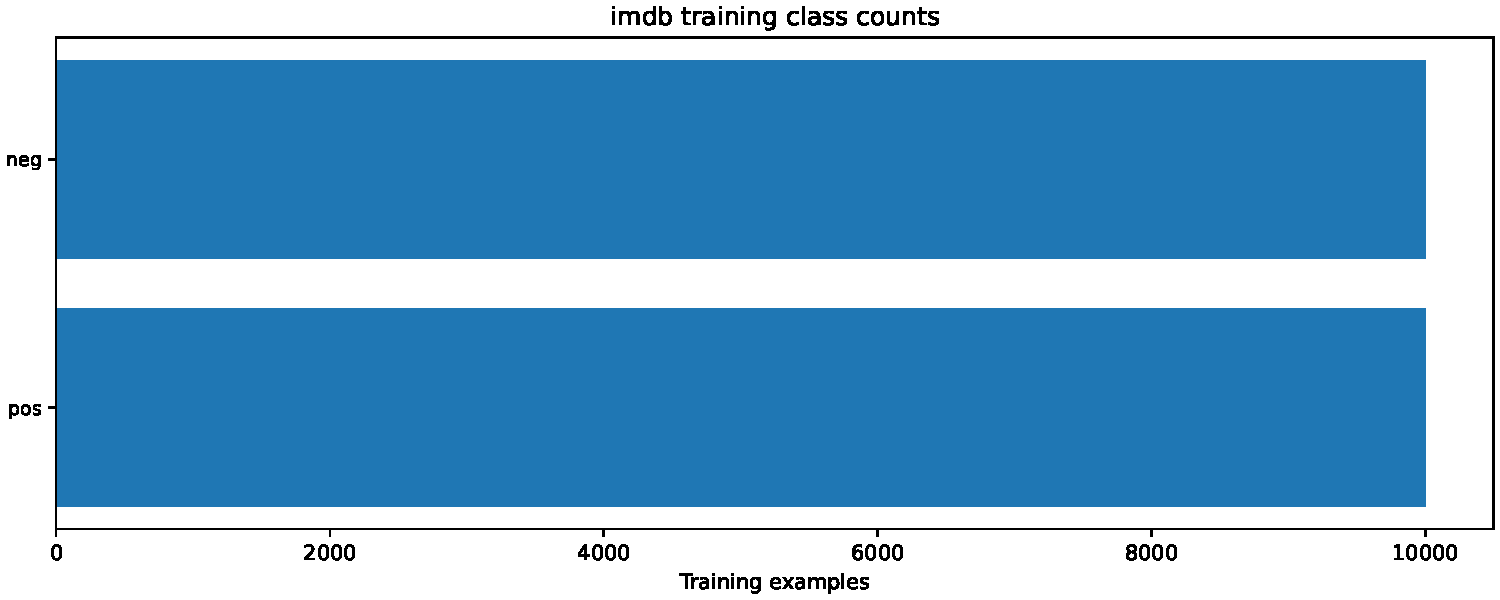
\includegraphics[width=.96\linewidth,height=90mm,keepaspectratio]{figures/imdb/class_counts.pdf}
\caption{IMDb training class frequencies.}\end{figure}


\begin{figure}[htbp]\centering
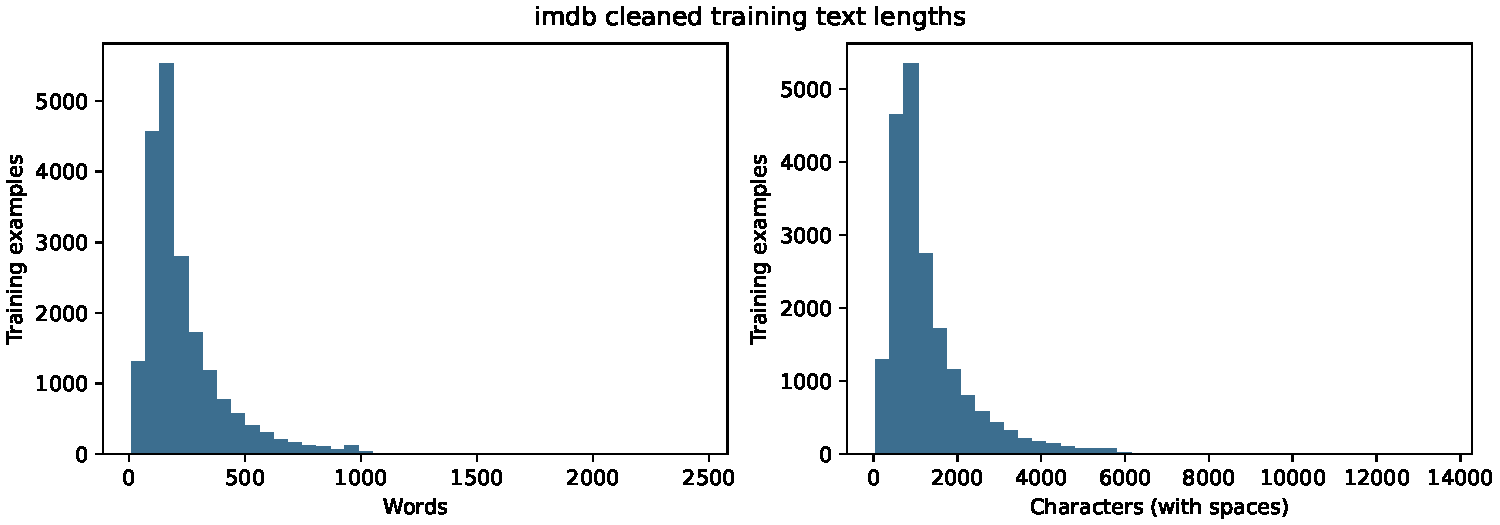
\includegraphics[width=.96\linewidth,height=75mm,keepaspectratio]{figures/imdb/lengths.pdf}
\caption{imdb cleaned training text lengths.}\end{figure}


\begin{figure}[htbp]\centering
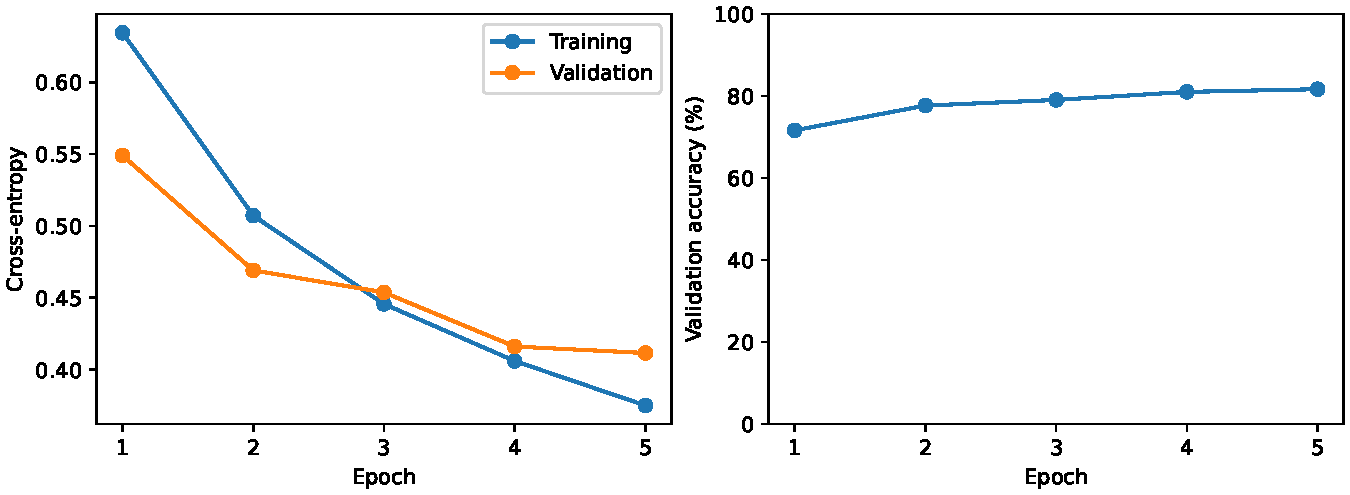
\includegraphics[width=.96\linewidth,height=75mm,keepaspectratio]{figures/imdb/learning_curves.pdf}
\caption{imdb randomly initialized Transformer learning curves.}\end{figure}






\clearpage

\subsection{banking77 results}

Training, validation, and test sizes are 8002, 2001, and 3080, respectively.

\begin{table}[htbp]\centering\small

\caption{Measured performance. Accuracies and macro-F1 are percentages. Time includes neural validation and checkpoint selection.}

\begin{tabular}{lrrrrr}\toprule

Model & Weights & Val.\ acc. & Test acc. & Test F1 & Seconds\\\midrule

baseline & 683,991 & 84.71 & 85.49 & 85.39 & 3.6\\

scratch & 139,149 & 51.17 & 49.06 & 46.06 & 17.5\\

transfer\_full & 4,395,853 & 84.01 & 83.12 & 82.40 & 83.2\\

transfer\_head & 9,933 & 15.34 & 13.02 & 9.38 & 22.1\\

transfer\_lower & 208,205 & 70.46 & 70.58 & 68.89 & 60.8\\

transfer\_upper & 208,205 & 72.26 & 69.90 & 68.55 & 51.8\\

\bottomrule\end{tabular}\end{table}

The randomly initialized Transformer changes test accuracy by -36.43 percentage points relative to the TF--IDF baseline. The baseline directly models word and bigram evidence, while the small Transformer learns its embeddings and contextual representation from the task training data. Input truncation and the fixed training budget may also affect the comparison. These possible explanations are not isolated causally by this experiment.

BANKING77 has 77 classes and only 103.9 training queries per class on average. Short domain-specific queries can provide useful word and bigram cues to the baseline, while the random Transformer must learn representations and a 77-way decision rule within the fixed epoch budget. The recorded truncation fractions help distinguish input-length effects from these factors.

The validation-selected fine-tuning configuration is \texttt{transfer\_full}, with test accuracy 83.12\%. Selection uses validation accuracy; test results are reported afterward.

The measured validation Pareto frontier contains transfer\_full, transfer\_head, transfer\_upper.

Full fine-tuning changes test accuracy by +70.10 percentage points relative to head-only training. The upper- and lower-block runs each unfreeze one encoder block, enabling a comparison at the same block budget.

Unfreezing the upper block changes validation accuracy by +1.80 percentage points relative to unfreezing the lower block. The corresponding test difference is -0.68 percentage points. This quantifies layer-position sensitivity for this checkpoint and training budget.

The fully fine-tuned pretrained model changes test accuracy by +34.06 percentage points relative to the random Transformer. Pretraining and architecture both differ in this comparison, so their effects are not isolated.

For \texttt{scratch}, 0.0\% of training texts exceed the input limit. The selected checkpoint is from epoch 5.

For \texttt{transfer\_full}, 0.0\% of training texts exceed the input limit. The selected checkpoint is from epoch 5.

For \texttt{transfer\_head}, 0.0\% of training texts exceed the input limit. The selected checkpoint is from epoch 5.

For \texttt{transfer\_lower}, 0.0\% of training texts exceed the input limit. The selected checkpoint is from epoch 5.

For \texttt{transfer\_upper}, 0.0\% of training texts exceed the input limit. The selected checkpoint is from epoch 5.

\par\medskip\noindent\begin{minipage}{\linewidth}

\paragraph{Example errors: baseline}

\begin{itemize}

\item True: card\_arrival; predicted: card\_linking. "How do I locate my card?..."

\item True: card\_arrival; predicted: transfer\_not\_received\_by\_recipient. "I ordered a card but it has not arrived. Help please!..."

\end{itemize}

\end{minipage}\par

\par\medskip\noindent\begin{minipage}{\linewidth}

\paragraph{Example errors: scratch}

\begin{itemize}

\item True: card\_arrival; predicted: card\_linking. "How do I locate my card?..."

\item True: card\_arrival; predicted: card\_not\_working. "I ordered a card but it has not arrived. Help please!..."

\end{itemize}

\end{minipage}\par

\par\medskip\noindent\begin{minipage}{\linewidth}

\paragraph{Example errors: transfer\_full}

\begin{itemize}

\item True: card\_arrival; predicted: card\_delivery\_estimate. "Is there a way to know when my card will arrive?..."

\item True: card\_arrival; predicted: card\_delivery\_estimate. "When will I get my card?..."

\end{itemize}

\end{minipage}\par

\par\medskip\noindent\begin{minipage}{\linewidth}

\paragraph{Example errors: transfer\_head}

\begin{itemize}

\item True: card\_arrival; predicted: verify\_top\_up. "How do I locate my card?..."

\item True: card\_arrival; predicted: wrong\_amount\_of\_cash\_received. "I still have not received my new card, I ordered over a week ago...."

\end{itemize}

\end{minipage}\par

\par\medskip\noindent\begin{minipage}{\linewidth}

\paragraph{Example errors: transfer\_lower}

\begin{itemize}

\item True: card\_arrival; predicted: card\_linking. "How do I locate my card?..."

\item True: card\_arrival; predicted: card\_delivery\_estimate. "Is there a way to know when my card will arrive?..."

\end{itemize}

\end{minipage}\par

\par\medskip\noindent\begin{minipage}{\linewidth}

\paragraph{Example errors: transfer\_upper}

\begin{itemize}

\item True: card\_arrival; predicted: lost\_or\_stolen\_card. "How do I locate my card?..."

\item True: card\_arrival; predicted: card\_delivery\_estimate. "Is there a way to know when my card will arrive?..."

\end{itemize}

\end{minipage}\par

\begin{figure}[htbp]\centering
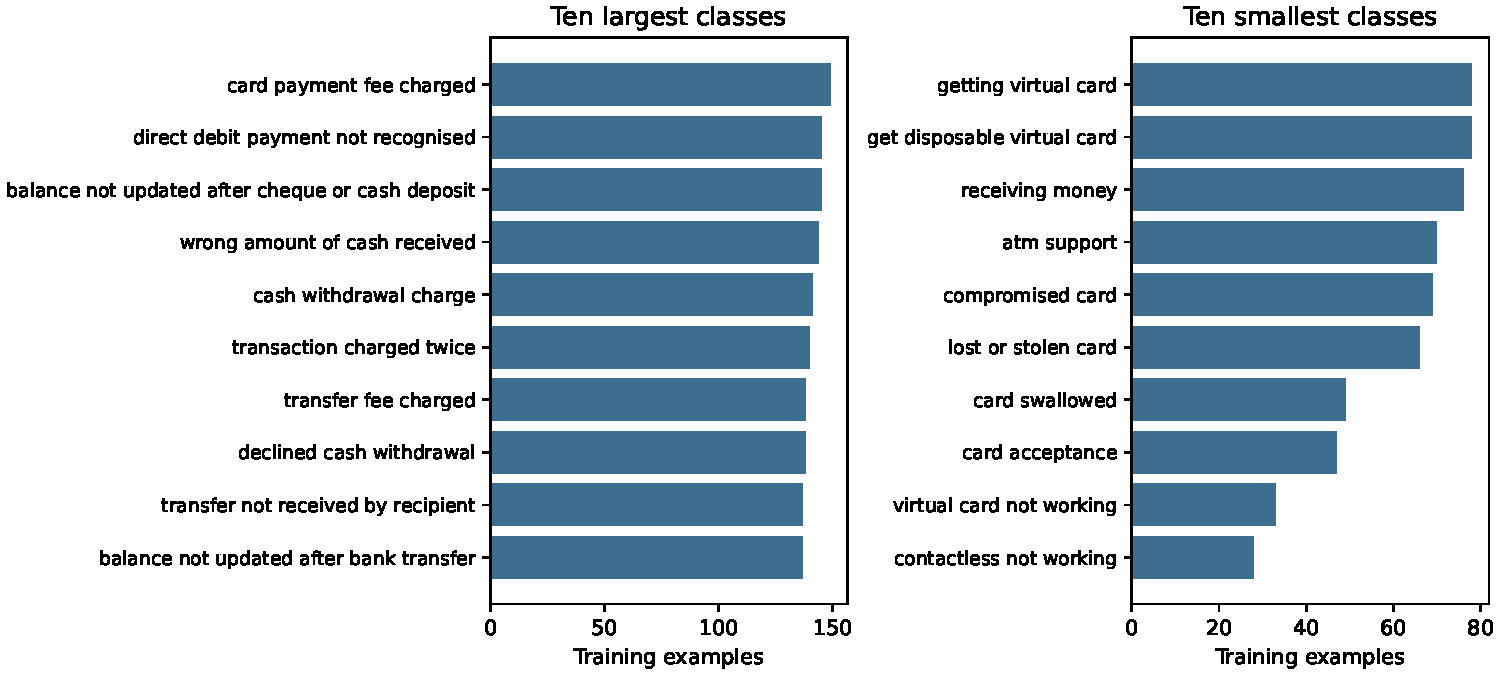
\includegraphics[width=.96\linewidth,height=90mm,keepaspectratio]{figures/banking77/class_overview.pdf}
\caption{BANKING77 ten largest and ten smallest training classes. The complete 77-class plot is saved separately as class\_counts.pdf.}\end{figure}


\begin{figure}[htbp]\centering
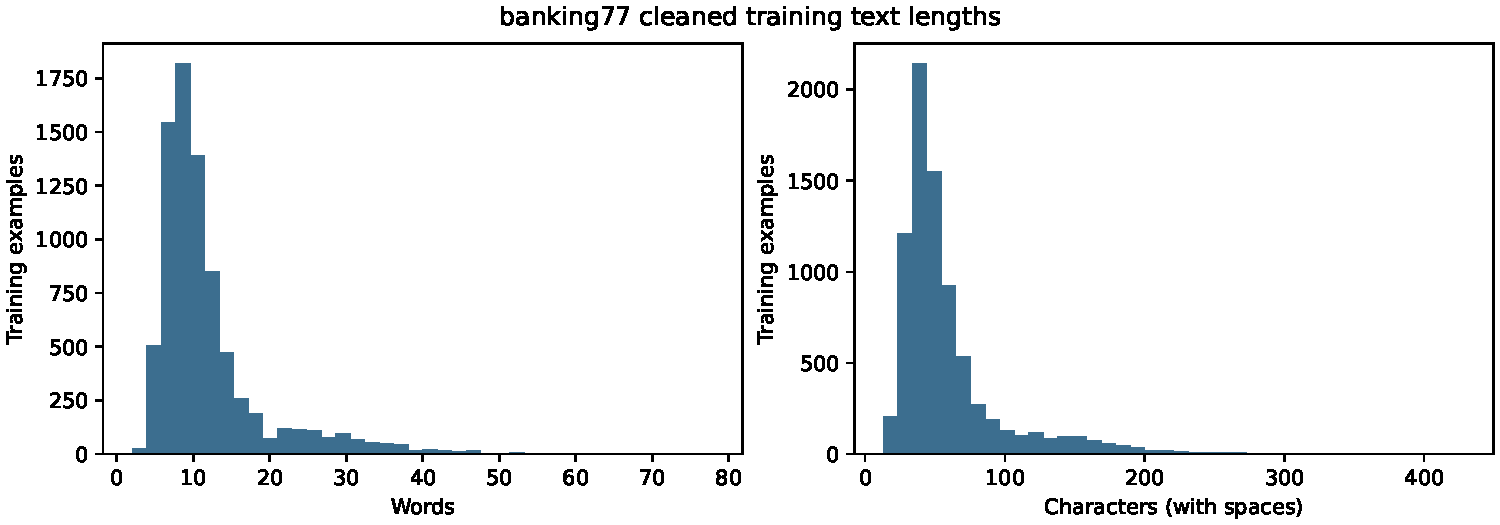
\includegraphics[width=.96\linewidth,height=75mm,keepaspectratio]{figures/banking77/lengths.pdf}
\caption{banking77 cleaned training text lengths.}\end{figure}


\begin{figure}[htbp]\centering
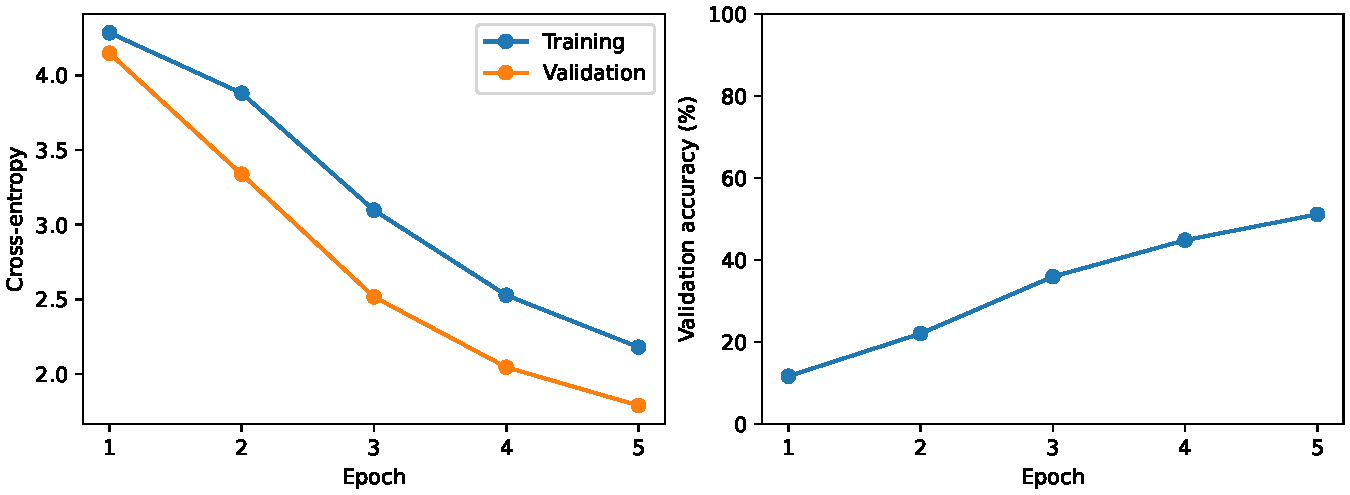
\includegraphics[width=.96\linewidth,height=75mm,keepaspectratio]{figures/banking77/learning_curves.pdf}
\caption{banking77 randomly initialized Transformer learning curves.}\end{figure}


\begin{figure}[htbp]\centering
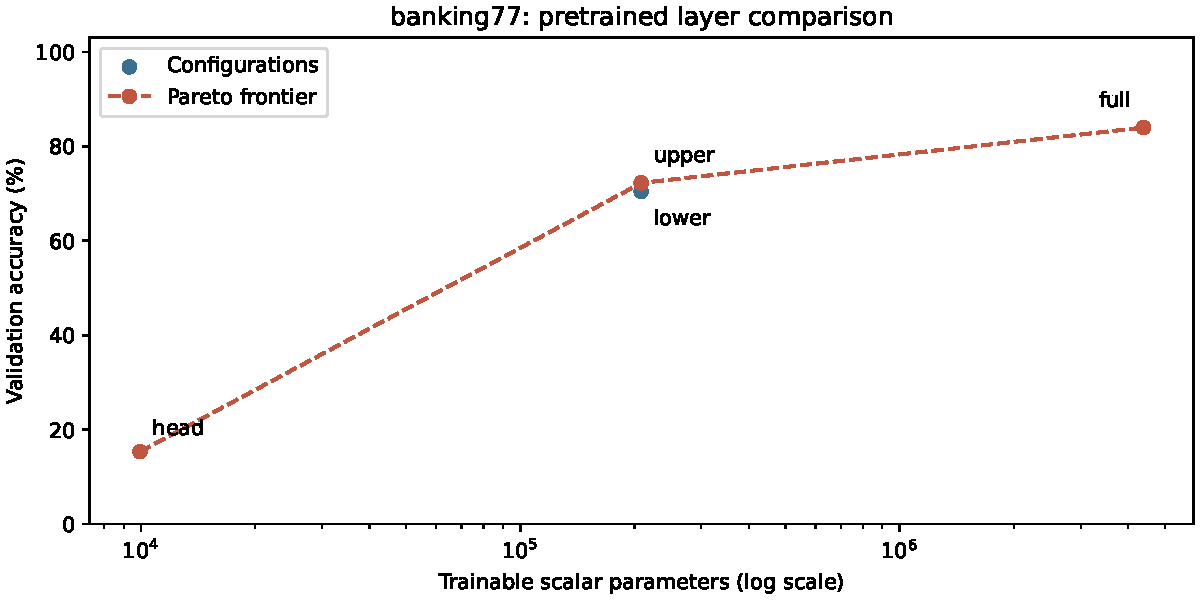
\includegraphics[width=.96\linewidth,height=75mm,keepaspectratio]{figures/banking77/pareto_validation.pdf}
\caption{banking77 validation Pareto frontier used for configuration comparison.}\end{figure}


\begin{figure}[htbp]\centering
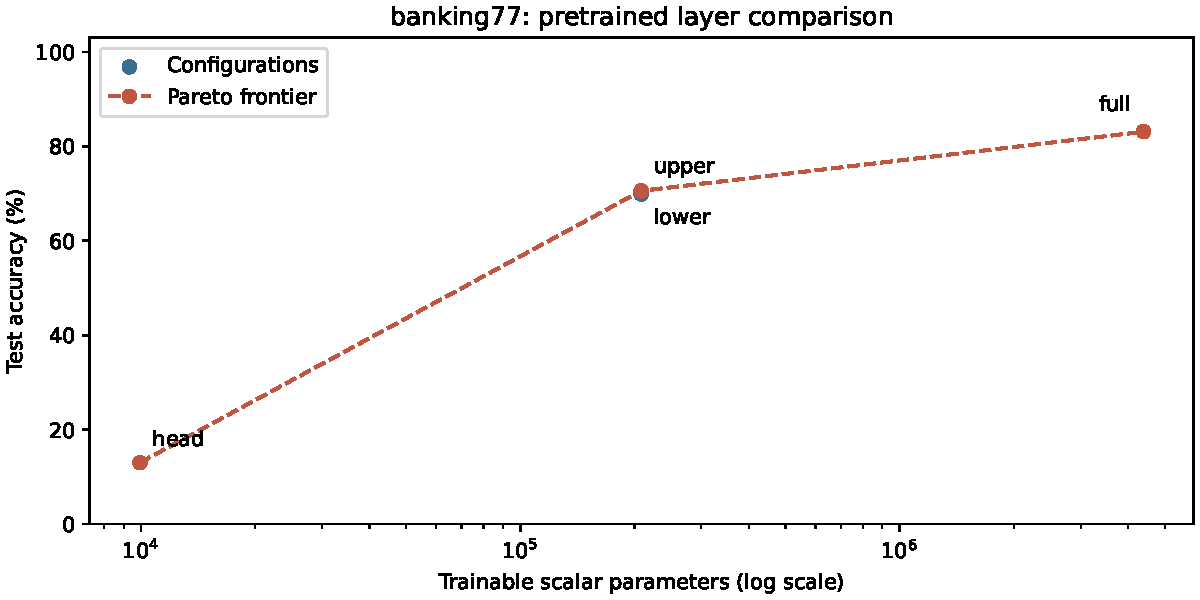
\includegraphics[width=.96\linewidth,height=75mm,keepaspectratio]{figures/banking77/pareto_test.pdf}
\caption{banking77 test accuracy versus trained weights; descriptive evaluation.}\end{figure}


\clearpage

\section{Conclusions and limitations}

Results use one random seed, one fixed hyperparameter budget, and a compact pretrained BERT checkpoint. Accuracy differences do not establish that one architecture is universally better. Broader learning-rate searches, repeated seeds, and larger checkpoints could change the ranking. Fine-tuning importance is assessed through the tested frozen-layer configurations.

For imdb, the highest validation accuracy among completed models is obtained by \texttt{baseline}. Its held-out test accuracy is 89.88\%.

For banking77, the highest validation accuracy among completed models is obtained by \texttt{baseline}. Its held-out test accuracy is 85.49\%.

\section{Reproducibility and repository files}
\texttt{Code\_Week\_2.py} is the command-line entry point.
The \texttt{week5} package contains independent implementation modules.
The \texttt{--part} option supports IMDb, BANKING77, transfer learning,
data preparation, and report generation separately.
Completed experiment outputs are reused when rerunning the same
configuration. A changed configuration requires a separate output
directory.

Results include per-run configuration, dataset metadata, environment
versions, metrics, validation/test predictions, classification reports,
training histories, checkpoints, parameter inventories, and PDF plots.
Checkpoints contain the selected state and reconstruction metadata.
The report tables and measured comparisons are generated from these
saved metrics. Runs use a single seed; repeated-seed uncertainty
estimation is a possible extension.
The commands and module layout are documented in the repository README.

\textbf{Repository}\quad
\url{https://github.com/Tuomashui/ADAMLY_project2}

\begin{thebibliography}{9}
\bibitem{banking77}
PolyAI. \emph{BANKING77 dataset}.
\url{https://huggingface.co/datasets/PolyAI/banking77}.
\bibitem{models}
Hugging Face. \emph{Pretrained models (assignment catalogue)}.
\url{https://huggingface.co/transformers/v1.2.0/pretrained_models.html}.
\bibitem{berttiny}
Prajjwal Bhargava. \emph{BERT-tiny pretrained checkpoint}.
\url{https://huggingface.co/prajjwal1/bert-tiny}.
\end{thebibliography}
\end{document}
